\section{Simple Reflex Agent}


\begin{figure}[H]
    \centering
    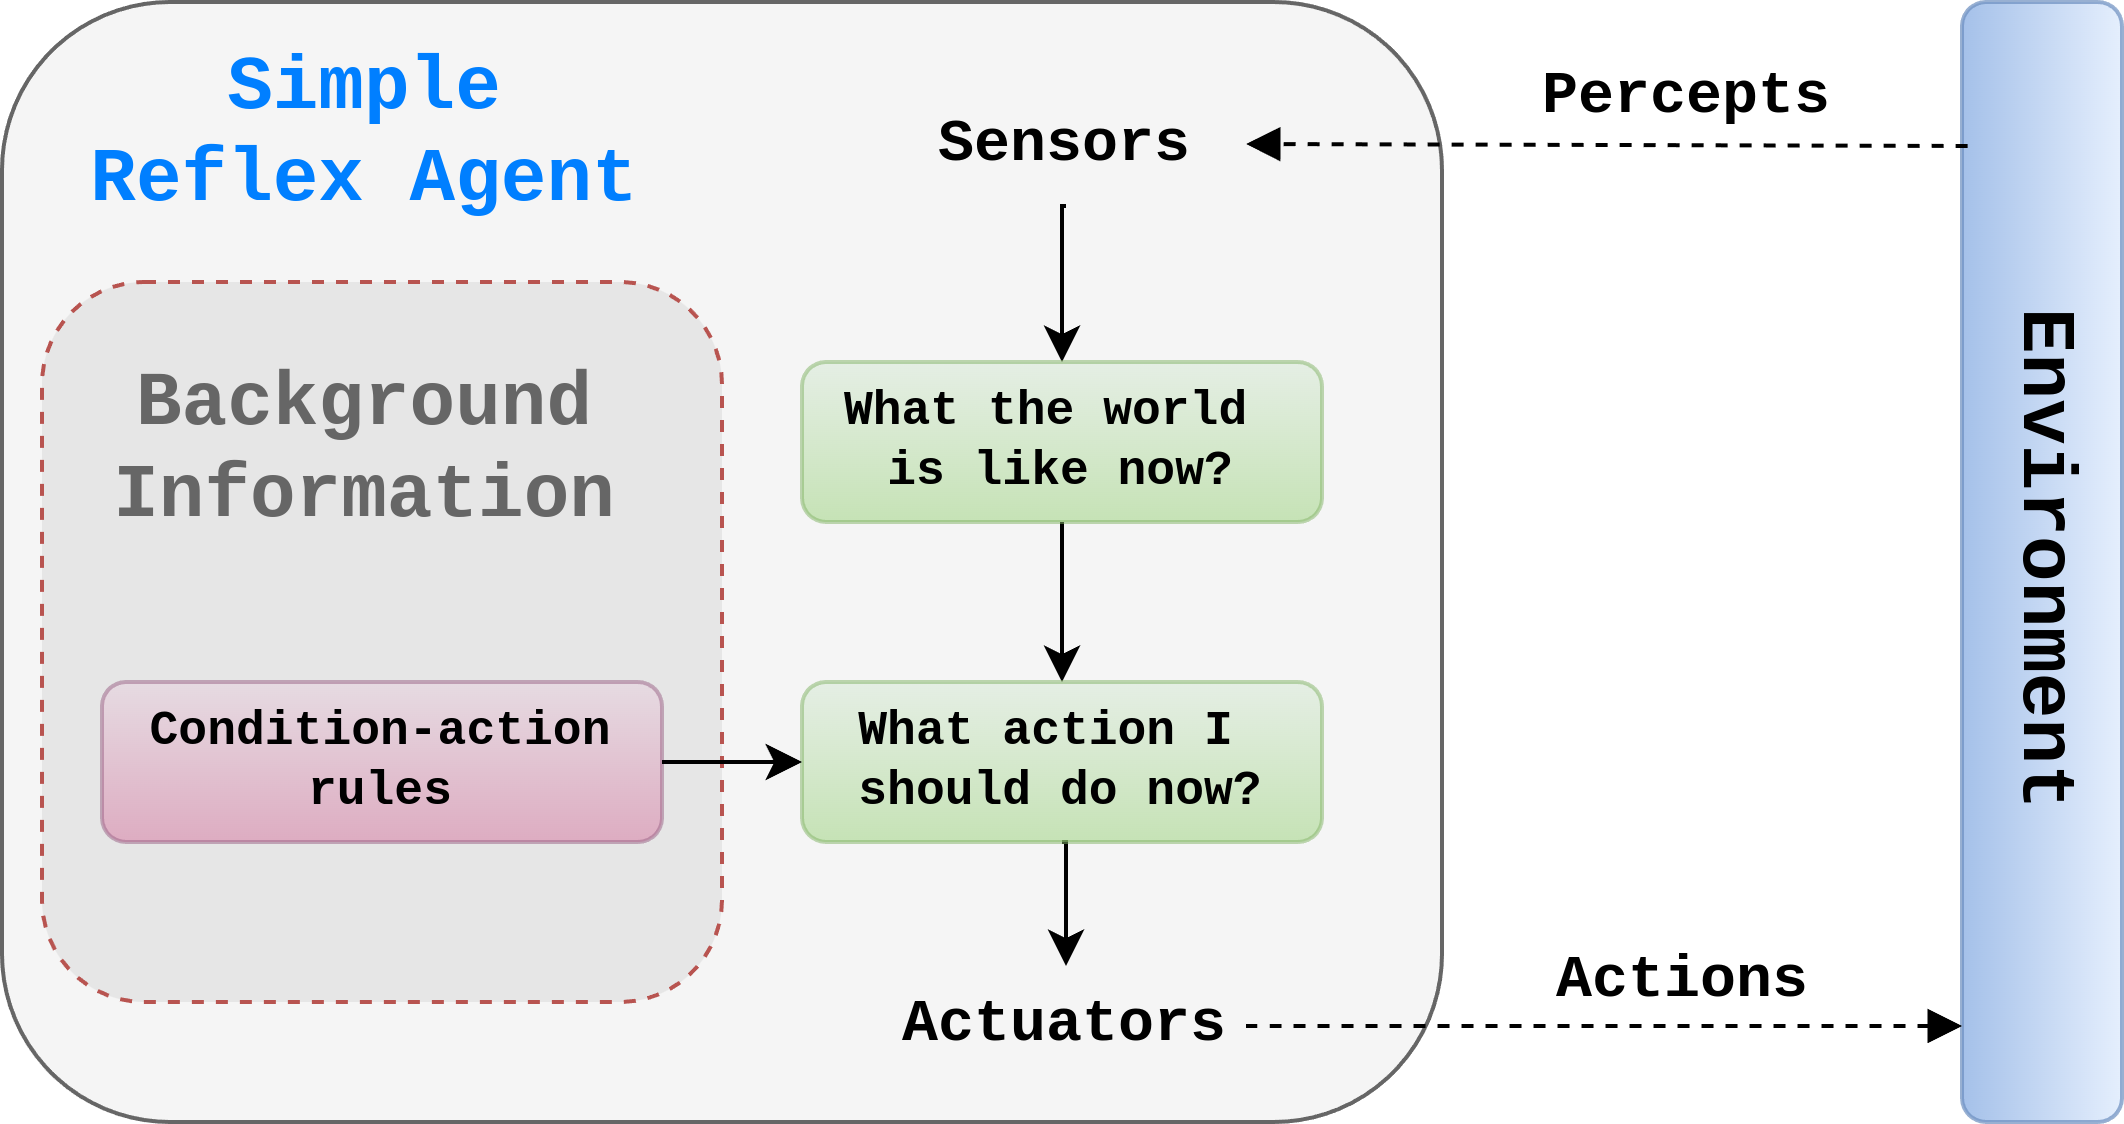
\includegraphics[
        width=0.5\linewidth, 
        height=4cm, 
        keepaspectratio
    ]{images/artificial-intelligence/ai-agents/agents-Simple-reflex-agent.png}
    \caption*{Schematic diagram of a simple reflex agent. \cite{common/online/tools/draw.io}}
\end{figure}

\begin{enumerate}[itemsep=0.2cm]
    \item simplest kind of agent
    \hfill \cite{ai/book/Artificial-Intelligence-A-Modern-Approach/Russell-Norvig}

    \item These agents select actions on the basis of the \textit{current} percept, ignoring the rest of the percept history.
    \hfill \cite{ai/book/Artificial-Intelligence-A-Modern-Approach/Russell-Norvig}

    \item \textbf{condition-action rule/ situation-action rules/ productions/ if-then rules}:\\
    A condition-action rule is a basic decision-making structure used in reflex agents and rule-based systems.
    \hfill \cite{ai/book/Artificial-Intelligence-A-Modern-Approach/Russell-Norvig, common/online/chatgpt}

    \item the description in terms of “rules” and “matching” is purely conceptual; actual implementations can be as simple as a collection of logic gates implementing a Boolean circuit.
    \hfill \cite{ai/book/Artificial-Intelligence-A-Modern-Approach/Russell-Norvig}

    \item \textbf{Disadvantage}: limited intelligence
    \hfill \cite{ai/book/Artificial-Intelligence-A-Modern-Approach/Russell-Norvig}

    \item \textbf{Disadvantage}: will work only if the correct decision can be made on the basis of only the current percept—that is, only if the environment is fully observable. Even a little bit of un-observability can cause serious trouble.
    \hfill \cite{ai/book/Artificial-Intelligence-A-Modern-Approach/Russell-Norvig}

\end{enumerate}


\vspace{0.5cm}


\begin{algorithm}[H]
    \caption{\textsc{Simple-Reflex-Agent}: It acts according to a rule whose condition matches the current state, as defined by the percept. \cite{ai/book/Artificial-Intelligence-A-Modern-Approach/Russell-Norvig}}

    \SetKwFunction{FUNCTION}{\textsc{Simple-Reflex-Agent}}
    \SetKwProg{Fn}{function}{ returns \normalfont an action}{end}
    \Fn{\FUNCTION{ percept }}{
        \textbf{persistent}: $rules$, a set of condition-action rules \\
        \ \\
        $state$ $\gets$ \textsc{Interpret-Input}( $percept$ )\\
        $rule$ $\gets$ \textsc{Rule-Match}( $state,\ rules$ ) \\
        $action$ $\gets$ $rule$.\textsc{Action} \\
        \Return $action$
    }
\end{algorithm}

\vspace{0.3cm}

\begin{customArrayStretch}{1.2}
\begin{longtable}{l p{12cm} l}

\textsc{Interpret-Input} & 
    generates an abstracted description of the current state from the percept &
    \cite{ai/book/Artificial-Intelligence-A-Modern-Approach/Russell-Norvig} \\

\textsc{Rule-Match} & 
    returns the first rule in the set of rules that matches the given state description &
    \cite{ai/book/Artificial-Intelligence-A-Modern-Approach/Russell-Norvig} \\

\end{longtable}
\end{customArrayStretch}









